\documentclass[a4paper, 11pt, titlepage]{article}
\usepackage{fancyhdr}
\usepackage{graphicx}
\usepackage{imakeidx}
\usepackage{makeidx}
\usepackage{mathtools}
\usepackage[spanish]{babel}
\usepackage{eurosym}
\usepackage{hyperref}
\usepackage{amssymb}
\usepackage{listings}
\usepackage{xcolor}

\setcounter{secnumdepth}{5}
\setcounter{tocdepth}{5}

\title{Criptografía y Esteganografía práctica sobre el entorno GNU/Linux}
\author{Francisco Javier Balón Aguilar}

\begin{document}

\maketitle
\renewcommand{\contentsname}{Índice}
\tableofcontents
\newpage

\section{Criptografía práctica sobre entorno GNU/Linux}

    \subsection{GnuPG (gpg)}
        
    GnuPG, a veces denominado simplemente gpg (siglas de GNU Privacy Guard) es un derivado libre
    de PGP. Su utilidad es la de cifrar y firmar digitalmente. gpg soporta tanto cifrado simétrico 
    como cifrado asimétrico.

    gpg tiene un repositorio de claves, llamado \textbf{anillo de claves} 
    donde almacena todas las claves que tenemos en nuestro sistema; sean privadas o públicas.

    Los \textbf{servidores de claves} ayudan a difundir las claves públicas 
    de forma que podamos compartirlas fácilmente para que otros usuarios puedan utilizarlas y
    cifrar con ellas.

    \subsubsection{Cifrado simétrico}

        El cifrado simétrico es sencillo; se utiliza la misma clave para cifrar y para descifrar.
        Es rápido de procesar y sencillo de usar, como contraposición, tiene la desventaja de la 
        comunicación de la clave\footnote{
            Tanto $A$ como $B$ deben conocer la misma clave. Por lo que si $A$ cifra un texto con
            la clave $123$, debe en algún momento comunicarla a $B$ para que éste pueda descifrarla.
            En esta comunicación encontramos un posible vector de ataque para obtener la clave.
        }.

        El uso de gpg con cifrado simétrico es muy sencillo. Simplemente llamamos a un texto sin cifrar
        con el parámetro $-c$ (crypt, cifrar) lo que generará un archivo en formato \textit{.gpg} cifrado
        por defecto con el algoritmo AES con la clave proporcionada (véase figuras \ref{crypt01} y 
        \ref{crypt02}).

        \begin{figure}[htp]
            \centering
            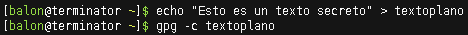
\includegraphics[width=0.8\textwidth]{resources/crypt01.png}
            \caption{Cifrado simétrico de archivo de texto.}
            \label{crypt01}
        \end{figure}

        \begin{figure}[htp]
            \centering
            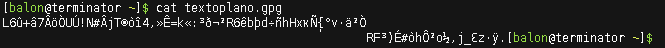
\includegraphics[width=0.8\textwidth]{resources/crypt02.png}
            \caption{Texto cifrado gpg.}
            \label{crypt02}
        \end{figure}

        Para descifrarlo, simplemente hay que pasarle a gpg el parámetro $-d$ (decrypt, descifrar) y el archivo 
        previamente cifrado (véase figura \ref{decrypt01}).

        \begin{figure}[htp]
            \centering
            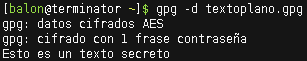
\includegraphics[width=0.5\textwidth]{resources/decrypt01.png}
            \caption{Texto descifrado con gpg con algoritmo simétrico AES.}
            \label{decrypt01}
        \end{figure}

    \subsubsection{Cifrado asimétrico}
        
        % TODO: genbeta.com/desarrollo/manual-de-gpg-cifra-y-envia-datos-de-forma-segura

        \subsubsection{Generación de par de claves}

        \subsubsection{Exportación e importación de claves}

        \subsubsection{Cifrado con clave pública}

        \subsubsection{Descifrado con clave privada}

    \subsubsection{Firma digital de archivos}

        \paragraph{Verificación y descifrado de archivos firmados}

    \subsubsection{Confiabilidad de claves}

    \subsection{SSH}

    % TODO: solvetic.com/tutoriales/article/1815-el-manual-del-secure-shell/
    \subsubsection{El cliente SSH}
    \subsubsection{El servidor SSH}
    \subsubsection{Securización de SSH}
    \subsubsection{Autenticación mediante intercambio de claves asimétricas (RSA)}

        
    \subsubsection{Exportación e importación de claves}
    \subsubsection{Generación de \textit{passphrase} y asociación con \textit{ssh-agent}}
    \subsubsection{SCP} \label{scp}
    \subsubsection{SFTP}

    % TODO: profesionalreview.com/2016/09/10/como-encriptar-datos-en-linux-ubuntu-linux-mint
    \subsection{VeraCrypt}
    \subsection{Files}
    \subsection{LUKS}
    \subsection{eCryptfs}
    \subsection{AESCrypt}

\section{Esteganografía práctica sobre el entorno GNU/Linux}

    \subsection{Steghide}

    % TODO: 2daygeek.com/easy-way-hide-information-inside-image-and-sound-objects

\end{document}